\documentclass[twoside]{book}

% Packages required by doxygen
\usepackage{fixltx2e}
\usepackage{calc}
\usepackage{doxygen}
\usepackage[export]{adjustbox} % also loads graphicx
\usepackage{graphicx}
\usepackage[utf8]{inputenc}
\usepackage{makeidx}
\usepackage{multicol}
\usepackage{multirow}
\PassOptionsToPackage{warn}{textcomp}
\usepackage{textcomp}
\usepackage[nointegrals]{wasysym}
\usepackage[table]{xcolor}

% Font selection
\usepackage[T1]{fontenc}
\usepackage[scaled=.90]{helvet}
\usepackage{courier}
\usepackage{amssymb}
\usepackage{sectsty}
\renewcommand{\familydefault}{\sfdefault}
\allsectionsfont{%
  \fontseries{bc}\selectfont%
  \color{darkgray}%
}
\renewcommand{\DoxyLabelFont}{%
  \fontseries{bc}\selectfont%
  \color{darkgray}%
}
\newcommand{\+}{\discretionary{\mbox{\scriptsize$\hookleftarrow$}}{}{}}

% Page & text layout
\usepackage{geometry}
\geometry{%
  a4paper,%
  top=2.5cm,%
  bottom=2.5cm,%
  left=2.5cm,%
  right=2.5cm%
}
\tolerance=750
\hfuzz=15pt
\hbadness=750
\setlength{\emergencystretch}{15pt}
\setlength{\parindent}{0cm}
\setlength{\parskip}{3ex plus 2ex minus 2ex}
\makeatletter
\renewcommand{\paragraph}{%
  \@startsection{paragraph}{4}{0ex}{-1.0ex}{1.0ex}{%
    \normalfont\normalsize\bfseries\SS@parafont%
  }%
}
\renewcommand{\subparagraph}{%
  \@startsection{subparagraph}{5}{0ex}{-1.0ex}{1.0ex}{%
    \normalfont\normalsize\bfseries\SS@subparafont%
  }%
}
\makeatother

% Headers & footers
\usepackage{fancyhdr}
\pagestyle{fancyplain}
\fancyhead[LE]{\fancyplain{}{\bfseries\thepage}}
\fancyhead[CE]{\fancyplain{}{}}
\fancyhead[RE]{\fancyplain{}{\bfseries\leftmark}}
\fancyhead[LO]{\fancyplain{}{\bfseries\rightmark}}
\fancyhead[CO]{\fancyplain{}{}}
\fancyhead[RO]{\fancyplain{}{\bfseries\thepage}}
\fancyfoot[LE]{\fancyplain{}{}}
\fancyfoot[CE]{\fancyplain{}{}}
\fancyfoot[RE]{\fancyplain{}{\bfseries\scriptsize Generated by Doxygen }}
\fancyfoot[LO]{\fancyplain{}{\bfseries\scriptsize Generated by Doxygen }}
\fancyfoot[CO]{\fancyplain{}{}}
\fancyfoot[RO]{\fancyplain{}{}}
\renewcommand{\footrulewidth}{0.4pt}
\renewcommand{\chaptermark}[1]{%
  \markboth{#1}{}%
}
\renewcommand{\sectionmark}[1]{%
  \markright{\thesection\ #1}%
}

% Indices & bibliography
\usepackage{natbib}
\usepackage[titles]{tocloft}
\setcounter{tocdepth}{3}
\setcounter{secnumdepth}{5}
\makeindex

% Hyperlinks (required, but should be loaded last)
\usepackage{ifpdf}
\ifpdf
  \usepackage[pdftex,pagebackref=true]{hyperref}
\else
  \usepackage[ps2pdf,pagebackref=true]{hyperref}
\fi
\hypersetup{%
  colorlinks=true,%
  linkcolor=blue,%
  citecolor=blue,%
  unicode%
}

% Custom commands
\newcommand{\clearemptydoublepage}{%
  \newpage{\pagestyle{empty}\cleardoublepage}%
}

\usepackage{caption}
\captionsetup{labelsep=space,justification=centering,font={bf},singlelinecheck=off,skip=4pt,position=top}

%===== C O N T E N T S =====

\begin{document}

% Titlepage & ToC
\hypersetup{pageanchor=false,
             bookmarksnumbered=true,
             pdfencoding=unicode
            }
\pagenumbering{alph}
\begin{titlepage}
\vspace*{7cm}
\begin{center}%
{\Large My Project }\\
\vspace*{1cm}
{\large Generated by Doxygen 1.8.13}\\
\end{center}
\end{titlepage}
\clearemptydoublepage
\pagenumbering{roman}
\tableofcontents
\clearemptydoublepage
\pagenumbering{arabic}
\hypersetup{pageanchor=true}

%--- Begin generated contents ---
\chapter{CS 202 Semester Project (W\+OO)}
\label{index}\hypertarget{index}{}\subsection*{Group Members!}


\begin{DoxyItemize}
\item Aaron Garza
\item Garrett Weinert
\end{DoxyItemize}

\subsection*{Responsibilities\+:}

\paragraph*{Garrett W.}


\begin{DoxyItemize}
\item Creating classes to identify and load files from a directory
\item Creating user interface for user to input a directory and manage wav files
\item Creating a C\+SV exporter \paragraph*{Aaron G.}
\end{DoxyItemize}


\begin{DoxyItemize}
\item Creating class to read/write wav files of varying types (mono/stereo and varying bit depth)
\item Creating classes to add audio effects to loaded wav files
\item Creating methods to modify the metadata of a wav file
\end{DoxyItemize}

\subsection*{Design}



Our design uses a C\+LI for the user to access the various functions the program offers that can be operated. Using the C\+LI, the user may load in the \hyperlink{classWav}{Wav} files from an inputted directory. After the files are loaded in, the user can select either to process a particular wav file, or to edit the metadata of a particular wav file using the meta data type. Once the meta-\/data desired is selected and changed, the user can export the data to a csv file. Once the user is finished, they can exit the application using an \char`\"{}exit\char`\"{} command.

\subsection*{Challenges encountered\+:}


\begin{DoxyItemize}
\item Choosing the best method by which wav files should be handled depending on technical data
\item Organizing work among the team in an online environment where communication is made more difficult
\item Operating Doxygen without ability to make the Git\+Hub page. (Still remains in /docs) 
\end{DoxyItemize}
\chapter{Branches}
\label{md_CONTRIBUTING}
\Hypertarget{md_CONTRIBUTING}
Use feature branching to contribute to the project. This should keep conflicts to a minimal.

Our branch names will look something like\+:
\begin{DoxyItemize}
\item {\ttfamily master}\+: Branch reflecting the current working verions. Don\textquotesingle{}t commit directly to master. This will be our branch that pull requests are merged to. Code changes are made in branchs and merged into development using a pull request. Use the following format when naming branches\+:
\begin{DoxyItemize}
\item {\ttfamily feature/some-\/branch-\/feature-\/description}
\end{DoxyItemize}
\end{DoxyItemize}

\#\+General Flow
\begin{DoxyItemize}
\item When creating a new feature\+:
\end{DoxyItemize}
\begin{DoxyEnumerate}
\item Pull from master to get latest changes\+: {\ttfamily git pull origin master}.
\item Create a new branch and switch over to it\+: {\ttfamily git checkout -\/b feature/some-\/branch-\/feature-\/description}.
\item Do work on branch. You can view which branch you are on via\+: {\ttfamily git status}.
\item When you feel your work is complete, you can merge to master.
\begin{DoxyItemize}
\item Make sure your branch has the latest master changes\+: ``` git checkout origin master git pull origin master ``{\ttfamily }
\item {\ttfamily Switch back to your feature branch and merge in master.}git merge master{\ttfamily }
\item {\ttfamily Commit and push changes to github.}git push some-\/feature-\/branch`
\item Open a pull request via Git\+Hub and click merge.
\end{DoxyItemize}
\end{DoxyEnumerate}

This flow should prevent us from stepping on each others code and keeps all merge conflicts 
\chapter{Hierarchical Index}
\section{Class Hierarchy}
This inheritance list is sorted roughly, but not completely, alphabetically\+:\begin{DoxyCompactList}
\item \contentsline{section}{App}{\pageref{classApp}}{}
\item \contentsline{section}{Command}{\pageref{classCommand}}{}
\begin{DoxyCompactList}
\item \contentsline{section}{Edit\+Meta\+Command}{\pageref{classEditMetaCommand}}{}
\item \contentsline{section}{Export\+Command}{\pageref{classExportCommand}}{}
\item \contentsline{section}{Load\+Command}{\pageref{classLoadCommand}}{}
\item \contentsline{section}{Process\+Command}{\pageref{classProcessCommand}}{}
\end{DoxyCompactList}
\item \contentsline{section}{Command\+Parser}{\pageref{classCommandParser}}{}
\item \contentsline{section}{Exporter}{\pageref{classExporter}}{}
\begin{DoxyCompactList}
\item \contentsline{section}{Csv\+Exporter}{\pageref{classCsvExporter}}{}
\end{DoxyCompactList}
\item \contentsline{section}{I\+Processable}{\pageref{classIProcessable}}{}
\begin{DoxyCompactList}
\item \contentsline{section}{Echo}{\pageref{classEcho}}{}
\item \contentsline{section}{Noise\+Gate}{\pageref{classNoiseGate}}{}
\item \contentsline{section}{Normalizer}{\pageref{classNormalizer}}{}
\end{DoxyCompactList}
\item \contentsline{section}{Wav}{\pageref{classWav}}{}
\item \contentsline{section}{wav\+\_\+header}{\pageref{structwav__header}}{}
\item \contentsline{section}{Wav\+Loader}{\pageref{classWavLoader}}{}
\item \contentsline{section}{Wav\+Store}{\pageref{classWavStore}}{}
\end{DoxyCompactList}

\chapter{Class Index}
\section{Class List}
Here are the classes, structs, unions and interfaces with brief descriptions\+:\begin{DoxyCompactList}
\item\contentsline{section}{\hyperlink{classApp}{App} }{\pageref{classApp}}{}
\item\contentsline{section}{\hyperlink{classCommand}{Command} }{\pageref{classCommand}}{}
\item\contentsline{section}{\hyperlink{classCommandParser}{Command\+Parser} }{\pageref{classCommandParser}}{}
\item\contentsline{section}{\hyperlink{classCsvExporter}{Csv\+Exporter} }{\pageref{classCsvExporter}}{}
\item\contentsline{section}{\hyperlink{classEcho}{Echo} }{\pageref{classEcho}}{}
\item\contentsline{section}{\hyperlink{classEditMetaCommand}{Edit\+Meta\+Command} }{\pageref{classEditMetaCommand}}{}
\item\contentsline{section}{\hyperlink{classExportCommand}{Export\+Command} }{\pageref{classExportCommand}}{}
\item\contentsline{section}{\hyperlink{classExporter}{Exporter} }{\pageref{classExporter}}{}
\item\contentsline{section}{\hyperlink{classIProcessable}{I\+Processable} }{\pageref{classIProcessable}}{}
\item\contentsline{section}{\hyperlink{classLoadCommand}{Load\+Command} }{\pageref{classLoadCommand}}{}
\item\contentsline{section}{\hyperlink{classNoiseGate}{Noise\+Gate} }{\pageref{classNoiseGate}}{}
\item\contentsline{section}{\hyperlink{classNormalizer}{Normalizer} }{\pageref{classNormalizer}}{}
\item\contentsline{section}{\hyperlink{classProcessCommand}{Process\+Command} }{\pageref{classProcessCommand}}{}
\item\contentsline{section}{\hyperlink{classWav}{Wav} }{\pageref{classWav}}{}
\item\contentsline{section}{\hyperlink{structwav__header}{wav\+\_\+header} }{\pageref{structwav__header}}{}
\item\contentsline{section}{\hyperlink{classWavLoader}{Wav\+Loader} }{\pageref{classWavLoader}}{}
\item\contentsline{section}{\hyperlink{classWavStore}{Wav\+Store} }{\pageref{classWavStore}}{}
\end{DoxyCompactList}

\chapter{File Index}
\section{File List}
Here is a list of all documented files with brief descriptions\+:\begin{DoxyCompactList}
\item\contentsline{section}{{\bfseries echo.\+h} }{\pageref{echo_8h}}{}
\item\contentsline{section}{\hyperlink{main_8cpp}{main.\+cpp} }{\pageref{main_8cpp}}{}
\item\contentsline{section}{{\bfseries noisegate.\+h} }{\pageref{noisegate_8h}}{}
\item\contentsline{section}{{\bfseries normalizer.\+h} }{\pageref{normalizer_8h}}{}
\item\contentsline{section}{{\bfseries processor.\+h} }{\pageref{processor_8h}}{}
\item\contentsline{section}{{\bfseries Wav.\+h} }{\pageref{Wav_8h}}{}
\item\contentsline{section}{{\bfseries wavheader.\+h} }{\pageref{wavheader_8h}}{}
\end{DoxyCompactList}

\chapter{Class Documentation}
\hypertarget{classEcho}{}\section{Echo Class Reference}
\label{classEcho}\index{Echo@{Echo}}


{\ttfamily \#include $<$echo.\+h$>$}



Inheritance diagram for Echo\+:
\nopagebreak
\begin{figure}[H]
\begin{center}
\leavevmode
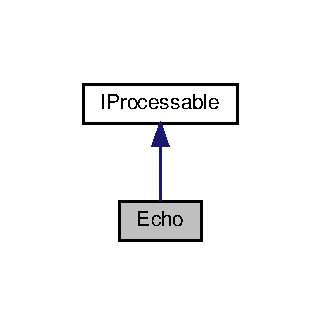
\includegraphics[width=154pt]{d1/dd3/classEcho__inherit__graph}
\end{center}
\end{figure}


Collaboration diagram for Echo\+:
\nopagebreak
\begin{figure}[H]
\begin{center}
\leavevmode
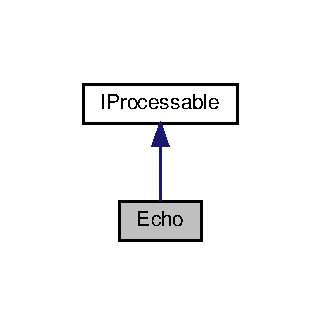
\includegraphics[width=154pt]{da/d44/classEcho__coll__graph}
\end{center}
\end{figure}
\subsection*{Public Member Functions}
\begin{DoxyCompactItemize}
\item 
\hyperlink{classEcho_a9531515ffab8be1e38cbdc0e0e9338a6}{Echo} (int delay)
\item 
void \hyperlink{classEcho_a1cdbe4bf78f5f6ac9b3609d9cd32de94}{process\+Buffer} (unsigned char $\ast$buffer, int buffer\+Size, int bit\+Depth, int num\+Channels) override
\end{DoxyCompactItemize}


\subsection{Detailed Description}
Class to add an echo effect to a .wav file 

\subsection{Constructor \& Destructor Documentation}
\mbox{\Hypertarget{classEcho_a9531515ffab8be1e38cbdc0e0e9338a6}\label{classEcho_a9531515ffab8be1e38cbdc0e0e9338a6}} 
\index{Echo@{Echo}!Echo@{Echo}}
\index{Echo@{Echo}!Echo@{Echo}}
\subsubsection{\texorpdfstring{Echo()}{Echo()}}
{\footnotesize\ttfamily Echo\+::\+Echo (\begin{DoxyParamCaption}\item[{int}]{delay }\end{DoxyParamCaption})}

Constructor for the \hyperlink{classEcho}{Echo} effect 
\begin{DoxyParams}{Parameters}
{\em delay} & -\/ the delay of each sample as an int \\
\hline
\end{DoxyParams}


\subsection{Member Function Documentation}
\mbox{\Hypertarget{classEcho_a1cdbe4bf78f5f6ac9b3609d9cd32de94}\label{classEcho_a1cdbe4bf78f5f6ac9b3609d9cd32de94}} 
\index{Echo@{Echo}!process\+Buffer@{process\+Buffer}}
\index{process\+Buffer@{process\+Buffer}!Echo@{Echo}}
\subsubsection{\texorpdfstring{process\+Buffer()}{processBuffer()}}
{\footnotesize\ttfamily void Echo\+::process\+Buffer (\begin{DoxyParamCaption}\item[{unsigned char $\ast$}]{buffer,  }\item[{int}]{buffer\+Size,  }\item[{int}]{bit\+Depth,  }\item[{int}]{num\+Channels }\end{DoxyParamCaption})\hspace{0.3cm}{\ttfamily [override]}, {\ttfamily [virtual]}}

Function that echoes each sample per user\textquotesingle{}s input 
\begin{DoxyParams}{Parameters}
{\em buffer} & -\/ buffer containing sound data \\
\hline
{\em buffer\+Size} & -\/ size of the buffer of sound data \\
\hline
{\em bit\+Depth} & -\/ bit depth of the .wav \\
\hline
{\em num\+Channels} & -\/ number of channels of the .wav \\
\hline
\end{DoxyParams}


Implements \hyperlink{classIProcessable_a818d23db44eefe70ef052c3ce9340f11}{I\+Processable}.



The documentation for this class was generated from the following files\+:\begin{DoxyCompactItemize}
\item 
echo.\+h\item 
echo.\+cpp\end{DoxyCompactItemize}

\hypertarget{classIProcessable}{}\section{I\+Processable Class Reference}
\label{classIProcessable}\index{I\+Processable@{I\+Processable}}


{\ttfamily \#include $<$processor.\+h$>$}



Inheritance diagram for I\+Processable\+:
\nopagebreak
\begin{figure}[H]
\begin{center}
\leavevmode
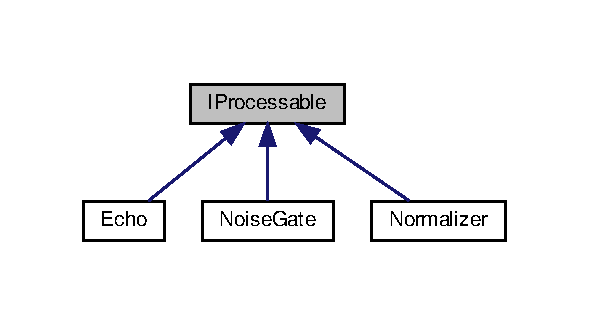
\includegraphics[width=283pt]{d5/dfc/classIProcessable__inherit__graph}
\end{center}
\end{figure}
\subsection*{Public Member Functions}
\begin{DoxyCompactItemize}
\item 
virtual void \hyperlink{classIProcessable_a818d23db44eefe70ef052c3ce9340f11}{process\+Buffer} (unsigned char $\ast$buffer, int buffer\+Size, int bit\+Depth, int num\+Channels)=0
\end{DoxyCompactItemize}


\subsection{Detailed Description}
Interface for adding various effects to .wav files 

\subsection{Member Function Documentation}
\mbox{\Hypertarget{classIProcessable_a818d23db44eefe70ef052c3ce9340f11}\label{classIProcessable_a818d23db44eefe70ef052c3ce9340f11}} 
\index{I\+Processable@{I\+Processable}!process\+Buffer@{process\+Buffer}}
\index{process\+Buffer@{process\+Buffer}!I\+Processable@{I\+Processable}}
\subsubsection{\texorpdfstring{process\+Buffer()}{processBuffer()}}
{\footnotesize\ttfamily virtual void I\+Processable\+::process\+Buffer (\begin{DoxyParamCaption}\item[{unsigned char $\ast$}]{buffer,  }\item[{int}]{buffer\+Size,  }\item[{int}]{bit\+Depth,  }\item[{int}]{num\+Channels }\end{DoxyParamCaption})\hspace{0.3cm}{\ttfamily [pure virtual]}}

Virtual function to be overridden by subclasses to add effects to .wav 

Implemented in \hyperlink{classEcho_a1cdbe4bf78f5f6ac9b3609d9cd32de94}{Echo}, \hyperlink{classNoiseGate_a7d58bdbe85f4e2709c77f5d3d5f34e09}{Noise\+Gate}, and \hyperlink{classNormalizer_ab17632635876ca5cf6da795525889761}{Normalizer}.



The documentation for this class was generated from the following file\+:\begin{DoxyCompactItemize}
\item 
processor.\+h\end{DoxyCompactItemize}

\hypertarget{classNoiseGate}{}\section{Noise\+Gate Class Reference}
\label{classNoiseGate}\index{Noise\+Gate@{Noise\+Gate}}


{\ttfamily \#include $<$noisegate.\+h$>$}



Inheritance diagram for Noise\+Gate\+:
\nopagebreak
\begin{figure}[H]
\begin{center}
\leavevmode
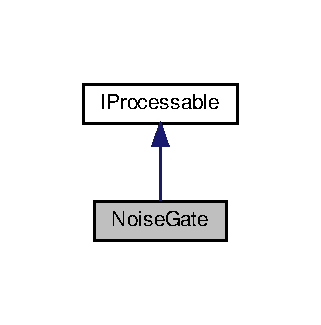
\includegraphics[width=154pt]{d5/d39/classNoiseGate__inherit__graph}
\end{center}
\end{figure}


Collaboration diagram for Noise\+Gate\+:
\nopagebreak
\begin{figure}[H]
\begin{center}
\leavevmode
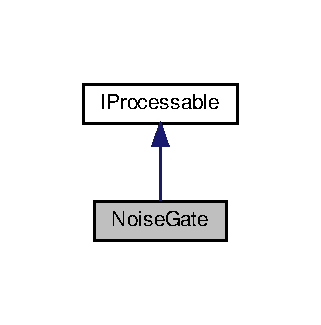
\includegraphics[width=154pt]{d8/da9/classNoiseGate__coll__graph}
\end{center}
\end{figure}
\subsection*{Public Member Functions}
\begin{DoxyCompactItemize}
\item 
\hyperlink{classNoiseGate_a5106cfbd673a9ba6faf5f283a92ebf93}{Noise\+Gate} (double threshold)
\item 
void \hyperlink{classNoiseGate_a7d58bdbe85f4e2709c77f5d3d5f34e09}{process\+Buffer} (unsigned char $\ast$buffer, int buffer\+Size, int bit\+Depth, int num\+Channels) override
\end{DoxyCompactItemize}


\subsection{Detailed Description}
Class to add a noise gate to a .wav file 

\subsection{Constructor \& Destructor Documentation}
\mbox{\Hypertarget{classNoiseGate_a5106cfbd673a9ba6faf5f283a92ebf93}\label{classNoiseGate_a5106cfbd673a9ba6faf5f283a92ebf93}} 
\index{Noise\+Gate@{Noise\+Gate}!Noise\+Gate@{Noise\+Gate}}
\index{Noise\+Gate@{Noise\+Gate}!Noise\+Gate@{Noise\+Gate}}
\subsubsection{\texorpdfstring{Noise\+Gate()}{NoiseGate()}}
{\footnotesize\ttfamily Noise\+Gate\+::\+Noise\+Gate (\begin{DoxyParamCaption}\item[{double}]{threshold }\end{DoxyParamCaption})}

Constructor for \hyperlink{classNoiseGate}{Noise\+Gate} effect 
\begin{DoxyParams}{Parameters}
{\em threshold} & -\/ percentage threshold for noise gating \\
\hline
\end{DoxyParams}


\subsection{Member Function Documentation}
\mbox{\Hypertarget{classNoiseGate_a7d58bdbe85f4e2709c77f5d3d5f34e09}\label{classNoiseGate_a7d58bdbe85f4e2709c77f5d3d5f34e09}} 
\index{Noise\+Gate@{Noise\+Gate}!process\+Buffer@{process\+Buffer}}
\index{process\+Buffer@{process\+Buffer}!Noise\+Gate@{Noise\+Gate}}
\subsubsection{\texorpdfstring{process\+Buffer()}{processBuffer()}}
{\footnotesize\ttfamily void Noise\+Gate\+::process\+Buffer (\begin{DoxyParamCaption}\item[{unsigned char $\ast$}]{buffer,  }\item[{int}]{buffer\+Size,  }\item[{int}]{bit\+Depth,  }\item[{int}]{num\+Channels }\end{DoxyParamCaption})\hspace{0.3cm}{\ttfamily [override]}, {\ttfamily [virtual]}}

Function that echoes each sample per user\textquotesingle{}s input 
\begin{DoxyParams}{Parameters}
{\em buffer} & -\/ buffer containing sound data \\
\hline
{\em buffer\+Size} & -\/ size of the buffer of sound data \\
\hline
{\em bit\+Depth} & -\/ bit depth of the .wav \\
\hline
{\em num\+Channels} & -\/ number of channels of the .wav \\
\hline
\end{DoxyParams}


Implements \hyperlink{classIProcessable_a818d23db44eefe70ef052c3ce9340f11}{I\+Processable}.



The documentation for this class was generated from the following files\+:\begin{DoxyCompactItemize}
\item 
noisegate.\+h\item 
noisegate.\+cpp\end{DoxyCompactItemize}

\hypertarget{classNormalizer}{}\section{Normalizer Class Reference}
\label{classNormalizer}\index{Normalizer@{Normalizer}}


{\ttfamily \#include $<$normalizer.\+h$>$}



Inheritance diagram for Normalizer\+:\nopagebreak
\begin{figure}[H]
\begin{center}
\leavevmode
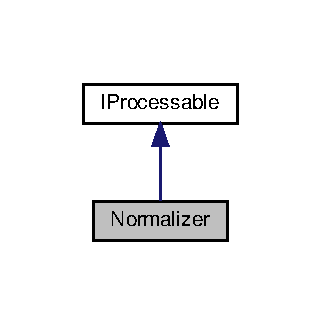
\includegraphics[width=154pt]{dd/d2d/classNormalizer__inherit__graph}
\end{center}
\end{figure}


Collaboration diagram for Normalizer\+:\nopagebreak
\begin{figure}[H]
\begin{center}
\leavevmode
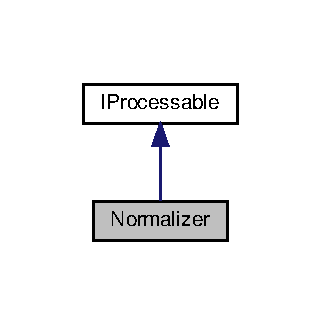
\includegraphics[width=154pt]{d9/da8/classNormalizer__coll__graph}
\end{center}
\end{figure}
\subsection*{Public Member Functions}
\begin{DoxyCompactItemize}
\item 
void \hyperlink{classNormalizer_ab17632635876ca5cf6da795525889761}{process\+Buffer} (unsigned char $\ast$buffer, int buffer\+Size, int bit\+Depth, int num\+Channels) override
\item 
{\footnotesize template$<$typename T $>$ }\\T \hyperlink{classNormalizer_a032dc937c5feeb167e5095f624434637}{get\+Max} (T first, T second)
\end{DoxyCompactItemize}


\subsection{Detailed Description}
Class to add a normalizer effect to .wav files 

\subsection{Member Function Documentation}
\mbox{\Hypertarget{classNormalizer_a032dc937c5feeb167e5095f624434637}\label{classNormalizer_a032dc937c5feeb167e5095f624434637}} 
\index{Normalizer@{Normalizer}!get\+Max@{get\+Max}}
\index{get\+Max@{get\+Max}!Normalizer@{Normalizer}}
\subsubsection{\texorpdfstring{get\+Max()}{getMax()}}
{\footnotesize\ttfamily template$<$typename T $>$ \\
T Normalizer\+::get\+Max (\begin{DoxyParamCaption}\item[{T}]{first,  }\item[{T}]{second }\end{DoxyParamCaption})\hspace{0.3cm}{\ttfamily [inline]}}

Function to find the max of two values 
\begin{DoxyParams}{Parameters}
{\em first} & -\/ first value to compare \\
\hline
{\em second} & -\/ second value to compare \\
\hline
\end{DoxyParams}
\mbox{\Hypertarget{classNormalizer_ab17632635876ca5cf6da795525889761}\label{classNormalizer_ab17632635876ca5cf6da795525889761}} 
\index{Normalizer@{Normalizer}!process\+Buffer@{process\+Buffer}}
\index{process\+Buffer@{process\+Buffer}!Normalizer@{Normalizer}}
\subsubsection{\texorpdfstring{process\+Buffer()}{processBuffer()}}
{\footnotesize\ttfamily void Normalizer\+::process\+Buffer (\begin{DoxyParamCaption}\item[{unsigned char $\ast$}]{buffer,  }\item[{int}]{buffer\+Size,  }\item[{int}]{bit\+Depth,  }\item[{int}]{num\+Channels }\end{DoxyParamCaption})\hspace{0.3cm}{\ttfamily [override]}, {\ttfamily [virtual]}}

Function that normalizes each sample dependent on sound data 
\begin{DoxyParams}{Parameters}
{\em buffer} & -\/ buffer containing sound data \\
\hline
{\em buffer\+Size} & -\/ size of the buffer of sound data \\
\hline
{\em bit\+Depth} & -\/ bit depth of the .wav \\
\hline
{\em num\+Channels} & -\/ number of channels of the .wav \\
\hline
\end{DoxyParams}


Implements \hyperlink{classIProcessable_a818d23db44eefe70ef052c3ce9340f11}{I\+Processable}.



The documentation for this class was generated from the following files\+:\begin{DoxyCompactItemize}
\item 
normalizer.\+h\item 
normalizer.\+cpp\end{DoxyCompactItemize}

\hypertarget{classWav}{}\section{Wav Class Reference}
\label{classWav}\index{Wav@{Wav}}


{\ttfamily \#include $<$Wav.\+h$>$}

\subsection*{Public Member Functions}
\begin{DoxyCompactItemize}
\item 
void \hyperlink{classWav_a1c4230cec49d30147a5b8a1950083f7c}{read\+File} (const std\+::string \&file\+Name)
\item 
void \hyperlink{classWav_ad86f4a21d36719ae375ea2586f9f591f}{write\+File} (const std\+::string \&out\+File\+Name)
\item 
virtual \hyperlink{classWav_a1510b246ba121b103a60b8e7839af25f}{$\sim$\+Wav} ()
\item 
unsigned char $\ast$ \hyperlink{classWav_a2daf07a90ed34789e3a1874973d9bd36}{get\+Buffer} ()
\item 
int \hyperlink{classWav_a71fdfa1d9f5e7c1b86f07bbff4249dca}{get\+Buffer\+Size} () const
\item 
int \hyperlink{classWav_ac09aa7f7d656a42bffdfafa737c0bce8}{getbit\+Depth} () const
\item 
int \hyperlink{classWav_a3be0de234388ed90f2039bf193214c02}{getnum\+Channels} () const
\item 
std\+::string \hyperlink{classWav_ab7049943bab3ee9bf8c6ca4043989f3c}{get\+Artist} () const
\item 
void \hyperlink{classWav_acf8f0bbb6e0791d1f0c083c6700e0607}{set\+Artist} (std\+::string x)
\item 
std\+::string \hyperlink{classWav_a8de3a1bd3cc70540869a2a42ace98022}{get\+Song\+Name} () const
\item 
void \hyperlink{classWav_a129cd26f79a06e932e5cefda0ecdb35a}{set\+Song\+Name} (std\+::string y)
\item 
void \hyperlink{classWav_aa05dac85e219a94afc6a6f38530306ce}{set\+File\+Path} (std\+::string file\+Path)
\item 
std\+::string \hyperlink{classWav_a2a0cddb7e39fa964ef46737fcfcb9372}{get\+File\+Path} ()
\end{DoxyCompactItemize}


\subsection{Detailed Description}
Class designed to read and write .wav files 

\subsection{Constructor \& Destructor Documentation}
\mbox{\Hypertarget{classWav_a1510b246ba121b103a60b8e7839af25f}\label{classWav_a1510b246ba121b103a60b8e7839af25f}} 
\index{Wav@{Wav}!````~Wav@{$\sim$\+Wav}}
\index{````~Wav@{$\sim$\+Wav}!Wav@{Wav}}
\subsubsection{\texorpdfstring{$\sim$\+Wav()}{~Wav()}}
{\footnotesize\ttfamily Wav\+::$\sim$\+Wav (\begin{DoxyParamCaption}{ }\end{DoxyParamCaption})\hspace{0.3cm}{\ttfamily [virtual]}}

Deconstructor for the \hyperlink{classWav}{Wav} object 

\subsection{Member Function Documentation}
\mbox{\Hypertarget{classWav_ab7049943bab3ee9bf8c6ca4043989f3c}\label{classWav_ab7049943bab3ee9bf8c6ca4043989f3c}} 
\index{Wav@{Wav}!get\+Artist@{get\+Artist}}
\index{get\+Artist@{get\+Artist}!Wav@{Wav}}
\subsubsection{\texorpdfstring{get\+Artist()}{getArtist()}}
{\footnotesize\ttfamily std\+::string Wav\+::get\+Artist (\begin{DoxyParamCaption}{ }\end{DoxyParamCaption}) const}

Returns the Artist held on a .wav file \mbox{\Hypertarget{classWav_ac09aa7f7d656a42bffdfafa737c0bce8}\label{classWav_ac09aa7f7d656a42bffdfafa737c0bce8}} 
\index{Wav@{Wav}!getbit\+Depth@{getbit\+Depth}}
\index{getbit\+Depth@{getbit\+Depth}!Wav@{Wav}}
\subsubsection{\texorpdfstring{getbit\+Depth()}{getbitDepth()}}
{\footnotesize\ttfamily int Wav\+::getbit\+Depth (\begin{DoxyParamCaption}{ }\end{DoxyParamCaption}) const}

Returns the bit\+Depth of a .wav file \mbox{\Hypertarget{classWav_a2daf07a90ed34789e3a1874973d9bd36}\label{classWav_a2daf07a90ed34789e3a1874973d9bd36}} 
\index{Wav@{Wav}!get\+Buffer@{get\+Buffer}}
\index{get\+Buffer@{get\+Buffer}!Wav@{Wav}}
\subsubsection{\texorpdfstring{get\+Buffer()}{getBuffer()}}
{\footnotesize\ttfamily unsigned char $\ast$ Wav\+::get\+Buffer (\begin{DoxyParamCaption}{ }\end{DoxyParamCaption})}

Returns the buffer of .wav sound data \mbox{\Hypertarget{classWav_a71fdfa1d9f5e7c1b86f07bbff4249dca}\label{classWav_a71fdfa1d9f5e7c1b86f07bbff4249dca}} 
\index{Wav@{Wav}!get\+Buffer\+Size@{get\+Buffer\+Size}}
\index{get\+Buffer\+Size@{get\+Buffer\+Size}!Wav@{Wav}}
\subsubsection{\texorpdfstring{get\+Buffer\+Size()}{getBufferSize()}}
{\footnotesize\ttfamily int Wav\+::get\+Buffer\+Size (\begin{DoxyParamCaption}{ }\end{DoxyParamCaption}) const}

Returns the size of the wav buffer \mbox{\Hypertarget{classWav_a2a0cddb7e39fa964ef46737fcfcb9372}\label{classWav_a2a0cddb7e39fa964ef46737fcfcb9372}} 
\index{Wav@{Wav}!get\+File\+Path@{get\+File\+Path}}
\index{get\+File\+Path@{get\+File\+Path}!Wav@{Wav}}
\subsubsection{\texorpdfstring{get\+File\+Path()}{getFilePath()}}
{\footnotesize\ttfamily std\+::string Wav\+::get\+File\+Path (\begin{DoxyParamCaption}{ }\end{DoxyParamCaption})}

Returns the full file path of source wav file. \mbox{\Hypertarget{classWav_a3be0de234388ed90f2039bf193214c02}\label{classWav_a3be0de234388ed90f2039bf193214c02}} 
\index{Wav@{Wav}!getnum\+Channels@{getnum\+Channels}}
\index{getnum\+Channels@{getnum\+Channels}!Wav@{Wav}}
\subsubsection{\texorpdfstring{getnum\+Channels()}{getnumChannels()}}
{\footnotesize\ttfamily int Wav\+::getnum\+Channels (\begin{DoxyParamCaption}{ }\end{DoxyParamCaption}) const}

Returns the number of channels of a .wav file \mbox{\Hypertarget{classWav_a8de3a1bd3cc70540869a2a42ace98022}\label{classWav_a8de3a1bd3cc70540869a2a42ace98022}} 
\index{Wav@{Wav}!get\+Song\+Name@{get\+Song\+Name}}
\index{get\+Song\+Name@{get\+Song\+Name}!Wav@{Wav}}
\subsubsection{\texorpdfstring{get\+Song\+Name()}{getSongName()}}
{\footnotesize\ttfamily std\+::string Wav\+::get\+Song\+Name (\begin{DoxyParamCaption}{ }\end{DoxyParamCaption}) const}

Returns the song name contained in a .wav file \mbox{\Hypertarget{classWav_a1c4230cec49d30147a5b8a1950083f7c}\label{classWav_a1c4230cec49d30147a5b8a1950083f7c}} 
\index{Wav@{Wav}!read\+File@{read\+File}}
\index{read\+File@{read\+File}!Wav@{Wav}}
\subsubsection{\texorpdfstring{read\+File()}{readFile()}}
{\footnotesize\ttfamily void Wav\+::read\+File (\begin{DoxyParamCaption}\item[{const std\+::string \&}]{file\+Name }\end{DoxyParamCaption})}

Reads in the technical data and metadata of a .wav file 
\begin{DoxyParams}{Parameters}
{\em file\+Name} & -\/ string of the .wav filename \\
\hline
\end{DoxyParams}
\mbox{\Hypertarget{classWav_acf8f0bbb6e0791d1f0c083c6700e0607}\label{classWav_acf8f0bbb6e0791d1f0c083c6700e0607}} 
\index{Wav@{Wav}!set\+Artist@{set\+Artist}}
\index{set\+Artist@{set\+Artist}!Wav@{Wav}}
\subsubsection{\texorpdfstring{set\+Artist()}{setArtist()}}
{\footnotesize\ttfamily void Wav\+::set\+Artist (\begin{DoxyParamCaption}\item[{std\+::string}]{x }\end{DoxyParamCaption})}

Changes the value of string Artist 
\begin{DoxyParams}{Parameters}
{\em x} & -\/ string to replace Artist value \\
\hline
\end{DoxyParams}
\mbox{\Hypertarget{classWav_aa05dac85e219a94afc6a6f38530306ce}\label{classWav_aa05dac85e219a94afc6a6f38530306ce}} 
\index{Wav@{Wav}!set\+File\+Path@{set\+File\+Path}}
\index{set\+File\+Path@{set\+File\+Path}!Wav@{Wav}}
\subsubsection{\texorpdfstring{set\+File\+Path()}{setFilePath()}}
{\footnotesize\ttfamily void Wav\+::set\+File\+Path (\begin{DoxyParamCaption}\item[{std\+::string}]{file\+Path }\end{DoxyParamCaption})}

Sets the full file path of source wav file. 
\begin{DoxyParams}{Parameters}
{\em file\+Path} & -\/ string path of wav file name. \\
\hline
\end{DoxyParams}
\mbox{\Hypertarget{classWav_a129cd26f79a06e932e5cefda0ecdb35a}\label{classWav_a129cd26f79a06e932e5cefda0ecdb35a}} 
\index{Wav@{Wav}!set\+Song\+Name@{set\+Song\+Name}}
\index{set\+Song\+Name@{set\+Song\+Name}!Wav@{Wav}}
\subsubsection{\texorpdfstring{set\+Song\+Name()}{setSongName()}}
{\footnotesize\ttfamily void Wav\+::set\+Song\+Name (\begin{DoxyParamCaption}\item[{std\+::string}]{y }\end{DoxyParamCaption})}

Changes value of string song\+Name 
\begin{DoxyParams}{Parameters}
{\em y} & -\/ string to replace song\+Name value \\
\hline
\end{DoxyParams}
\mbox{\Hypertarget{classWav_ad86f4a21d36719ae375ea2586f9f591f}\label{classWav_ad86f4a21d36719ae375ea2586f9f591f}} 
\index{Wav@{Wav}!write\+File@{write\+File}}
\index{write\+File@{write\+File}!Wav@{Wav}}
\subsubsection{\texorpdfstring{write\+File()}{writeFile()}}
{\footnotesize\ttfamily void Wav\+::write\+File (\begin{DoxyParamCaption}\item[{const std\+::string \&}]{out\+File\+Name }\end{DoxyParamCaption})}

Writes the technical data and metadata to a .wav file 
\begin{DoxyParams}{Parameters}
{\em out\+File\+Name} & -\/ Name of the file being output \\
\hline
\end{DoxyParams}


The documentation for this class was generated from the following files\+:\begin{DoxyCompactItemize}
\item 
Wav.\+h\item 
Wav.\+cpp\end{DoxyCompactItemize}

\hypertarget{structwav__header}{}\section{wav\+\_\+header Struct Reference}
\label{structwav__header}\index{wav\+\_\+header@{wav\+\_\+header}}
\subsection*{Public Attributes}
\begin{DoxyCompactItemize}
\item 
\mbox{\Hypertarget{structwav__header_a977b8193bf1f39dbd815c6210f0bb6c6}\label{structwav__header_a977b8193bf1f39dbd815c6210f0bb6c6}} 
char {\bfseries riff\+\_\+header} \mbox{[}4\mbox{]}
\item 
\mbox{\Hypertarget{structwav__header_a89a86a26a94e726411e34517bfc9105e}\label{structwav__header_a89a86a26a94e726411e34517bfc9105e}} 
int {\bfseries wav\+\_\+size}
\item 
\mbox{\Hypertarget{structwav__header_a0dc0cff34ad7fe5e59c5cbcee1640354}\label{structwav__header_a0dc0cff34ad7fe5e59c5cbcee1640354}} 
char {\bfseries wave\+\_\+header} \mbox{[}4\mbox{]}
\item 
\mbox{\Hypertarget{structwav__header_a4039d1e8e91d7940aa45a29aad27b4ce}\label{structwav__header_a4039d1e8e91d7940aa45a29aad27b4ce}} 
char {\bfseries fmt\+\_\+header} \mbox{[}4\mbox{]}
\item 
\mbox{\Hypertarget{structwav__header_a5fb4363d52bbff51ca2e8884408208c6}\label{structwav__header_a5fb4363d52bbff51ca2e8884408208c6}} 
int {\bfseries fmt\+\_\+chunk\+\_\+size}
\item 
\mbox{\Hypertarget{structwav__header_a94c9ee0387f846c47eb9e97636994d93}\label{structwav__header_a94c9ee0387f846c47eb9e97636994d93}} 
short {\bfseries audio\+\_\+format}
\item 
\mbox{\Hypertarget{structwav__header_a625d84de0f598e50c072d725f6e3b6b8}\label{structwav__header_a625d84de0f598e50c072d725f6e3b6b8}} 
short {\bfseries num\+\_\+channels}
\item 
\mbox{\Hypertarget{structwav__header_a0632019c676aa88f0351c0ab11461de0}\label{structwav__header_a0632019c676aa88f0351c0ab11461de0}} 
int {\bfseries sample\+\_\+rate}
\item 
\mbox{\Hypertarget{structwav__header_a8330740d45200d6aee4ba54fc0d834d8}\label{structwav__header_a8330740d45200d6aee4ba54fc0d834d8}} 
int {\bfseries byte\+\_\+rate}
\item 
\mbox{\Hypertarget{structwav__header_a2672b73c81973008677db6349fbc232a}\label{structwav__header_a2672b73c81973008677db6349fbc232a}} 
short {\bfseries sample\+\_\+alignment}
\item 
\mbox{\Hypertarget{structwav__header_a63fa60069060bae97c8a64c5b37afa23}\label{structwav__header_a63fa60069060bae97c8a64c5b37afa23}} 
short {\bfseries bit\+\_\+depth}
\item 
\mbox{\Hypertarget{structwav__header_ae43fac12459053e98a80e3879c5cd2a7}\label{structwav__header_ae43fac12459053e98a80e3879c5cd2a7}} 
char {\bfseries data\+\_\+header} \mbox{[}4\mbox{]}
\item 
\mbox{\Hypertarget{structwav__header_a3eeeca270947eab7c7aaee61bbee9b0e}\label{structwav__header_a3eeeca270947eab7c7aaee61bbee9b0e}} 
int {\bfseries data\+\_\+bytes}
\end{DoxyCompactItemize}


The documentation for this struct was generated from the following file\+:\begin{DoxyCompactItemize}
\item 
wavheader.\+h\end{DoxyCompactItemize}

\chapter{File Documentation}
\hypertarget{main_8cpp}{}\section{main.\+cpp File Reference}
\label{main_8cpp}\index{main.\+cpp@{main.\+cpp}}
{\ttfamily \#include \char`\"{}app/\+App.\+h\char`\"{}}\newline
Include dependency graph for main.\+cpp\+:
\nopagebreak
\begin{figure}[H]
\begin{center}
\leavevmode
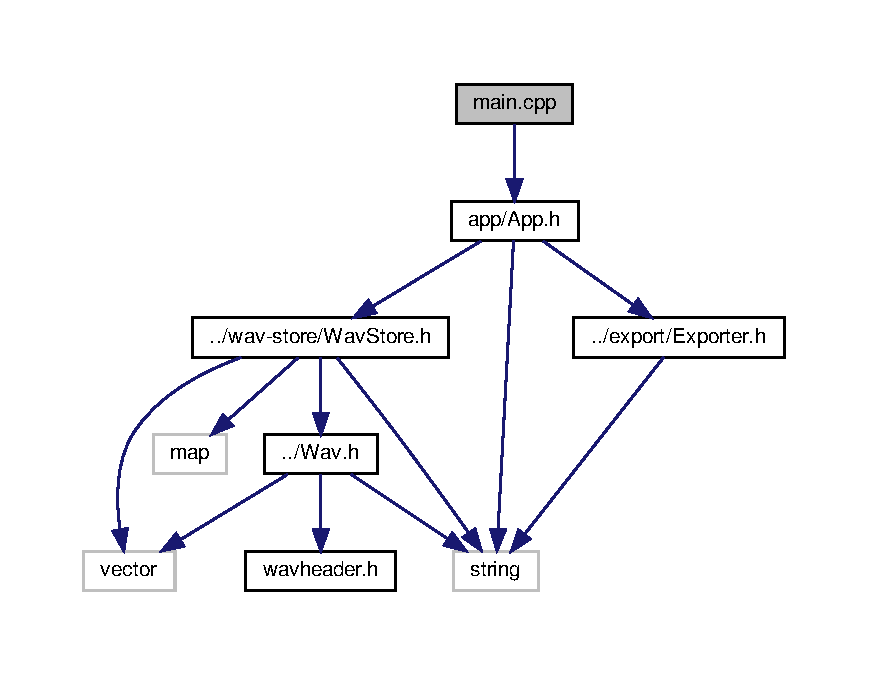
\includegraphics[width=350pt]{da/dce/main_8cpp__incl}
\end{center}
\end{figure}
\subsection*{Functions}
\begin{DoxyCompactItemize}
\item 
void \hyperlink{main_8cpp_ad9d0e397081801b3c81f84aef014b9ca}{fn} ()
\begin{DoxyCompactList}\small\item\em The function bar. \end{DoxyCompactList}\item 
\mbox{\Hypertarget{main_8cpp_ae66f6b31b5ad750f1fe042a706a4e3d4}\label{main_8cpp_ae66f6b31b5ad750f1fe042a706a4e3d4}} 
int {\bfseries main} ()
\end{DoxyCompactItemize}


\subsection{Function Documentation}
\mbox{\Hypertarget{main_8cpp_ad9d0e397081801b3c81f84aef014b9ca}\label{main_8cpp_ad9d0e397081801b3c81f84aef014b9ca}} 
\index{main.\+cpp@{main.\+cpp}!fn@{fn}}
\index{fn@{fn}!main.\+cpp@{main.\+cpp}}
\subsubsection{\texorpdfstring{fn()}{fn()}}
{\footnotesize\ttfamily void fn (\begin{DoxyParamCaption}{ }\end{DoxyParamCaption})}



The function bar. 

This function does something which is doing nothing. So this text is totally senseless and you really do not need to read this, because this text is basically saying nothing.

\begin{DoxyNote}{Note}
This text shall only show you, how such a "note" section is looking. There is nothing which really needs your notice, so you do not really need to read this section.
\end{DoxyNote}

\begin{DoxyParams}[1]{Parameters}
\mbox{\tt in}  & {\em a} & Description of parameter a. \\
\hline
\mbox{\tt out}  & {\em b} & Description of the parameter b. \\
\hline
\mbox{\tt in,out}  & {\em c} & Description of the parameter c.\\
\hline
\end{DoxyParams}
\begin{DoxyReturn}{Returns}
The error return code of the function.
\end{DoxyReturn}

\begin{DoxyRetVals}{Return values}
{\em E\+R\+R\+\_\+\+S\+U\+C\+C\+E\+SS} & The function is successfully executed \\
\hline
{\em E\+R\+R\+\_\+\+F\+A\+I\+L\+U\+RE} & An error occurred \\
\hline
\end{DoxyRetVals}

%--- End generated contents ---

% Index
\backmatter
\newpage
\phantomsection
\clearemptydoublepage
\addcontentsline{toc}{chapter}{Index}
\printindex

\end{document}
